\documentclass[12pt,a4paper]{report} % Sử dụng lớp 'report' để hỗ trợ các chương \chapter

% --- GÓI CẤU HÌNH VĂN BẢN & NGÔN NGỮ ---
\usepackage[utf8]{inputenc} % Đã sửa cú pháp utf8
\usepackage[english]{babel} % Ngôn ngữ báo cáo tiếng Anh chuẩn Academic
\usepackage{geometry}
\geometry{
    a4paper,
    top=25mm,
    bottom=25mm,
    left=30mm,
    right=20mm
}
\usepackage{setspace}
\onehalfspacing % Dãn dòng 1.5 chuẩn báo cáo

% --- GÓI HỖ TRỢ BẢNG BỂ, HÌNH ẢNH & MÃ NGUỒN ---
\usepackage{tabularx}   % Bảng tự động dãn cột (dùng trong workflow, testing)
\usepackage{longtable}  % Bảng dài nhiều trang (dùng trong Test Cases, Requirements)
\usepackage{booktabs}   % Kẻ bảng chuẩn Academic
\usepackage{xcolor}     % Nhãn màu PASS/FAIL/CRITICAL
\usepackage{graphicx}   % Chèn hình ảnh
\usepackage{listings}   % Hỗ trợ định dạng Code Snippet/JSON/YAML

% --- GÓI HỖ TRỢ LIÊN KẾT & TRÍCH DẪN ---
\usepackage{hyperref}
\hypersetup{
    colorlinks=true,
    linkcolor=blue,
    filecolor=magenta,      
    urlcolor=cyan,
    pdftitle={LivingDocs - Software Project Report},
    pdfpagemode=FullScreen, % Đã sửa tham số pdfpagemode
}

% --- THÔNG TIN TRANG BÌA ---
\title{
    \Huge \textbf{LivingDocs System} \\[0.5em]
    \Large Automated Documentation Generation \& Synchronization Platform \\[1.5em]
    \large Capstone Project Report
}
\author{
    \textbf{Software Engineering Project Team} \\
    \small Department of Computer Science \& Software Engineering
}
\date{\today}

\begin{document}

% --- TRANG BÌA ---
\maketitle
\thispagestyle{empty}

% --- MỤC LỤC ---
\newpage
\pagenumbering{roman}
\tableofcontents 
\newpage

% --- NỘI DUNG CHÍNH (CÁC CHƯƠNG .TEX) ---
\pagenumbering{arabic}

\section{Introduction}

\subsection{Project Overview}
In modern software development, technical documentation plays a crucial role in helping development, testing, and maintenance teams work effectively. However, in many real-world projects, documentation is often not updated promptly when source code changes, leading to inconsistencies between documentation and the deployed system.

To address this issue, the team proposes building the \textbf{LivingDocs} system – an intelligent platform for software documentation management, capable of directly connecting to GitHub to track source code changes and automatically suggest documentation updates using Artificial Intelligence (AI).

LivingDocs helps reduce manual workload in the documentation process while improving accuracy, traceability, and consistency between source code and technical documentation.

\subsection{Objectives}
The objectives of the system include:
\begin{itemize}
    \item Automatically detect source code changes on GitHub.
    \item Generate technical documentation using AI.
    \item Detect inconsistencies between source code and documentation.
    \item Support collaboration among multiple team members in the same project.
    \item Manage documentation versions and change history.
\end{itemize}

\subsection{Project Scope}
The LivingDocs system focuses on supporting software development teams in building and maintaining technical documentation.  
The main functions include:
\begin{itemize}
    \item GitHub Integration.
    \item AI Documentation Generation.
    \item Automatic Documentation Update.
    \item Documentation Drift Detection.
    \item Knowledge Base Management.
    \item Workflow Collaboration.
    \item System Administration.
    \item Testing and Deployment.
\end{itemize}

\chapter{Software Requirements Specification}

\section{Introduction}

\subsection{Document Purpose}
This document specifies the software requirements for the \textbf{LivingDocs -- Design and Implementation of an AI-Assisted Self-Updating Document System for Engineering Teams} platform.

LivingDocs is an AI-powered documentation maintenance platform engineered to detect documentation drift, automatically generate and update technical documentation from source code, and enforce a multi-tiered Human-in-the-Loop review workflow.

This specification focuses on:
\begin{itemize}
	\item User requirements and target personas.
	\item Functional Requirements (FR).
	\item Non-Functional Requirements (NFR).
	\item User roles and access control mechanisms.
	\item Documentation drift detection and management workflows.
	\item Verification, auditing, and document versioning controls.
\end{itemize}

\textit{Note: This document excludes low-level architectural blueprints, database schema design, or specific code implementation details, which are addressed in subsequent system design modules.}

\section{System Scope}
LivingDocs automates the continuous maintenance of technical documentation across software engineering projects.

Key capabilities include:
\begin{itemize}
	\item Seamless integration with GitHub repositories via OAuth and Webhooks.
	\item Continuous ingestion of commit updates and Pull Requests.
	\item Automated static code and AST analysis.
	\item Bidirectional mapping between code entities and documentation artifacts.
	\item Multi-classification of documentation drift (Referential, Signature, Semantic).
	\item AI-assisted document generation and context-aware auto-updates.
	\item Granular version history and complete audit traceability.
	\item Multi-tiered review workflows involving Staff Reviewers and Manager Approvers.
	\item Searchable Knowledge Base linking documentation directly to live code.
	\item System-wide governance and administrative controls.
\end{itemize}

\section{System Objectives}
The primary objectives of LivingDocs encompass:
\begin{itemize}
	\item Minimizing technical documentation debt in fast-paced development environments.
	\item Proactively identifying outdated or contradictory documentation.
	\item Detecting structural reference breaks as well as semantic behavioral shifts.
	\item Reducing manual overhead required for writing and updating technical docs.
	\item Ensuring high precision and global consistency across project documentation.
	\item Maintaining strict human governance over AI-generated outputs.
	\item Guaranteeing complete auditability and version rollback capabilities.
\end{itemize}

\section{Target User Personas}
The system defines five primary operational roles:

\begin{longtable}{p{4.5cm} p{9cm}}
	\toprule
	\textbf{Role} & \textbf{Description} \\
	\midrule
	\endhead
	
	Developer (Author) &
	Engineers who connect repositories, initiate AI documentation generation, review drift alerts, and submit documentation drafts for review. \\
	
	Staff (Reviewer) &
	Technical personnel responsible for conducting the initial technical review of AI-generated or auto-updated documentation. \\
	
	Manager (Approver) &
	Decision-makers responsible for final approval, publication, or direct repository commit authorization. \\
	
	Technical Lead / Owner &
	Administrators managing documentation standards, drift policies, custom templates, and quality compliance. \\
	
	Administrator &
	System administrators managing user accounts, RBAC policies, GitHub integration setups, and backend infrastructure. \\
	
	\bottomrule
\end{longtable}

\section{User Requirements}

\subsection{Developer (Author)}
Developers require the capability to:
\begin{itemize}
	\item Authenticate via credentials or GitHub OAuth.
	\item Manage personal profiles and notification preferences.
	\item Link GitHub accounts and select repositories for workspace ingestion.
	\item Monitor repository sync status and trigger manual re-synchronization.
	\item View ingested commits and Pull Requests.
	\item Generate technical documentation from source code via AI.
	\item Select customized documentation templates and preview draft outputs.
	\item Identify code entities lacking documentation coverage.
	\item Edit AI-generated drafts and inspect grounding evidence before submission.
	\item Submit drafts into review workflows and monitor progress.
	\item Inspect documentation drift alerts, severity levels, and associated diffs.
	\item Compare document versions and perform version rollbacks.
	\item Search the knowledge base for linked code entities and documentation.
\end{itemize}

\subsection{Staff (Reviewer)}
Staff members require the capability to:
\begin{itemize}
	\item Access a centralized review queue.
	\item Inspect documentation side-by-side with code grounding evidence.
	\item Compare proposed versions against the latest approved baseline.
	\item Verify compliance with designated documentation templates and code truth.
	\item Inline review comments, request modifications, or make minor corrections.
	\item Approve drafts for Manager escalation or reject drafts with actionable feedback.
	\item Filter, sort, and track historical review logs.
\end{itemize}

\subsection{Manager (Approver)}
Managers require the capability to:
\begin{itemize}
	\item Access high-priority approval queues containing Staff-reviewed docs.
	\item Review Staff feedback, change diffs, and complete audit trails.
	\item Grant final approval for automatic repository commits or public publishing.
	\item Reject submissions or mandate further revisions.
	\item Execute emergency rollbacks to prior approved versions.
	\item Configure approval policies based on drift severity (e.g., Critical drift).
	\item Delegate or reassign approval authority.
\end{itemize}

\subsection{Technical Lead / Documentation Owner}
Technical Leads require the capability to:
\begin{itemize}
	\item Organize and manage documentation collections and ownership.
	\item Define drift detection sensitivity thresholds and update policies.
	\item Monitor the Documentation Health Dashboard (coverage, freshness, drift metrics).
	\item View code-to-documentation dependency graphs.
	\item Export health compliance and audit reports.
	\item Create, clone, modify, and publish version-controlled documentation templates.
	\item Configure mandatory template headings, sections, and placeholders.
\end{itemize">}

\subsection{Administrator}
Administrators require the capability to:
\begin{itemize}
	\item Manage user accounts, roles, and granular RBAC permissions.
	\item Configure workspace configurations, GitHub Apps, OAuth credentials, and webhooks.
	\item Define supported programming languages and parser configurations.
	\item Set AI inference endpoints, token quotas, and vector indexing parameters.
	\item Monitor event processing pipelines, background jobs, and system health.
	\item Inspect system-wide administrative audit logs.
\end{itemize">}

\section{Functional Requirements}

\subsection{Account and Authentication}
\begin{longtable}{p{2cm} p{11.3cm}}
	\toprule
	\textbf{ID} & \textbf{Requirement Description} \\
	\midrule
	\endhead
	FR01 & The system shall allow users to register new accounts. \\
	FR02 & The system shall allow users to securely log in and log out. \\
	FR03 & The system shall support authentication via Email/Password and GitHub OAuth. \\
	FR04 & The system shall enable users to manage profiles and notification preferences. \\
	\bottomrule
\end{longtable}

\subsection{GitHub Integration}
\begin{longtable}{p{2cm} p{11.3cm}}
	\toprule
	\textbf{ID} & \textbf{Requirement Description} \\
	\midrule
	\endhead
	FR05 & The system shall allow developers to link GitHub accounts via OAuth2. \\
	FR06 & The system shall display requested access scopes and permissions. \\
	FR07 & The system shall allow users to select and import target repositories. \\
	FR08 & The system shall support disconnecting repositories and revoking access tokens. \\
	FR09 & The system shall display synchronization status, default branch, and last sync timestamp. \\
	FR10 & The system shall support manual trigger of repository re-synchronization. \\
	FR11 & The system shall track ingested commits and Pull Request events. \\
	FR12 & The system shall alert administrators upon Webhook or token expiration. \\
	\bottomrule
\end{longtable}

\subsection{AI Source-Code Reading \& Documentation Generation}
\begin{longtable}{p{2cm} p{11.3cm}}
	\toprule
	\textbf{ID} & \textbf{Requirement Description} \\
	\midrule
	\endhead
	FR13 & The system shall support doc generation at file, module, or repository levels. \\
	FR14 & The system shall analyze AST and code structure to synthesize documentation. \\
	FR15 & The system shall allow selecting predefined documentation templates. \\
	FR16 & The system shall identify code entities lacking documentation coverage. \\
	FR17 & The system shall provide a real-time preview of AI-generated drafts. \\
	FR18 & The system shall allow Developers to edit drafts prior to submission. \\
	FR19 & The system shall display grounding evidence (code references) for generated docs. \\
	FR20 & The system shall allow submitting generated drafts into the review workflow. \\
	FR21 & The system shall display the current workflow state of the document. \\
	\bottomrule
\end{longtable}

\subsection{Automatic Documentation Update}
\begin{longtable}{p{2cm} p{11.3cm}}
	\toprule
	\textbf{ID} & \textbf{Requirement Description} \\
	\midrule
	\endhead
	FR22 & The system shall detect affected documentation upon Pull Request or commit updates. \\
	FR23 & The system shall automatically generate updated document drafts and increment versions. \\
	FR24 & The system shall allow toggling auto-update features per repository or module. \\
	FR25 & The system shall provide side-by-side diff views between auto-updated drafts and published docs. \\
	FR26 & The system shall highlight specific triggering commits and diff chunks. \\
	FR27 & The system shall support accepting, editing, or dismissing auto-updated suggestions. \\
	FR28 & The system shall allow manual re-generation of documentation updates on demand. \\
	FR29 & The system shall support one-click rollbacks to pre-update states. \\
	\bottomrule
\end{longtable}

\subsection{Documentation Drift Detection and Review}
\begin{longtable}{p{2cm} p{11.3cm}}
	\toprule
	\textbf{ID} & \textbf{Requirement Description} \\
	\midrule
	\endhead
	FR30 & The system shall analyze Pull Request diffs to detect documentation drift. \\
	FR31 & The system shall present grounding evidence for every drift alert. \\
	FR32 & The system shall classify drift into Referential, Signature, or Semantic categories. \\
	FR33 & The system shall assign drift severity levels: Low, Medium, High, or Critical. \\
	FR34 & The system shall generate context-aware fix suggestions for detected drift. \\
	FR35 & The system shall support manual trigger of drift analysis for specific files or PRs. \\
	FR36 & The system shall maintain historical logs of drift occurrences and resolution actions. \\
	\bottomrule
\end{longtable}

\subsection{Change Logs and Version History}
\begin{longtable}{p{2cm} p{11.3cm}}
	\toprule
	\textbf{ID} & \textbf{Requirement Description} \\
	\midrule
	\endhead
	FR37 & The system shall record full change histories for every document. \\
	FR38 & The system shall allow comparing differences across any two arbitrary versions. \\
	FR39 & The system shall log acting user/role, timestamp, and trigger event for each version. \\
	FR40 & The system shall allow restoring or rolling back documents to previous versions. \\
	\bottomrule
\end{longtable}

\subsection{Knowledge Base}
\begin{longtable}{p{2cm} p{11.3cm}}
	\toprule
	\textbf{ID} & \textbf{Requirement Description} \\
	\midrule
	\endhead
	FR41 & The system shall provide full-text search across documentation and linked code entities. \\
	FR42 & The system shall render interactive dependency graphs between code and documentation. \\
	FR43 & The system shall allow bidirectional navigation between code files and docs. \\
	\bottomrule
\end{longtable}

\subsection{Review and Approval Workflows}
\begin{longtable}{p{2cm} p{11.3cm}}
	\toprule
	\textbf{ID} & \textbf{Requirement Description} \\
	\midrule
	\endhead
	FR44 & The system shall provide a dedicated Staff Review Queue. \\
	FR45 & Staff shall be able to inspect grounding evidence, change logs, and template rules. \\
	FR46 & Staff shall be able to approve, reject, inline-edit, or request revisions. \\
	FR47 & The system shall provide a Manager Approval Queue for Staff-approved documents. \\
	FR48 & Managers shall have final authority to publish or execute automated repository commits. \\
	FR49 & The system shall enforce mandatory approval rules before committing changes. \\
	FR50 & The system shall record complete, immutable audit logs of all approval decisions. \\
	\bottomrule
\end{longtable}

\subsection{Governance and Administration}
\begin{longtable}{p{2cm} p{11.3cm}}
	\toprule
	\textbf{ID} & \textbf{Requirement Description} \\
	\midrule
	\endhead
	FR51 & Tech Leads shall be able to configure drift detection thresholds and quality policies. \\
	FR52 & The system shall display real-time documentation health dashboards and freshness metrics. \\
	FR53 & Tech Leads shall be able to manage, version, and preview document templates. \\
	FR54 & Administrators shall manage RBAC permissions, language parsers, and AI settings. \\
	FR55 & Administrators shall monitor background processing pipelines, job statuses, and system health. \\
	\bottomrule
\end{longtable}

\section{Non-Functional Requirements}

\subsection{Performance}
\begin{longtable}{p{2cm} p{11.3cm}}
	\toprule
	\textbf{ID} & \textbf{Requirement Description} \\
	\midrule
	\endhead
	NFR01 & The system shall complete drift analysis for a PR within 2 minutes for repos up to 100k LOC. \\
	NFR02 & The system shall process at least 20 concurrent PR events without performance degradation. \\
	NFR03 & Standard API response times shall remain below 2 seconds under normal workload. \\
	NFR04 & Full-text search queries within the Knowledge Base shall return results within 1 second. \\
	\bottomrule
\end{longtable}

\subsection{Availability \& Scalability}
\begin{longtable}{p{2cm} p{11.3cm}}
	\toprule
	\textbf{ID} & \textbf{Requirement Description} \\
	\midrule
	\endhead
	NFR05 & The system shall maintain an operational uptime availability of at least 99.5\%. \\
	NFR06 & Background worker failures shall not impact user-facing web services. \\
	NFR07 & AI processing workers shall support horizontal auto-scaling based on queue depth. \\
	\bottomrule
\end{longtable}

\subsection{Security \& Reliability}
\begin{longtable}{p{2cm} p{11.3cm}}
	\toprule
	\textbf{ID} & \textbf{Requirement Description} \\
	\midrule
	\endhead
	NFR08 & All API endpoints and communications shall enforce HTTPS/TLS encryption. \\
	NFR09 & Access shall be strictly controlled via Role-Based Access Control (RBAC). \\
	NFR10 & Sensitive credentials and integration keys shall be encrypted at rest. \\
	NFR11 & System audit logs shall be immutable and retention-configurable. \\
	NFR12 & Drift detection algorithms shall yield deterministic evaluations for identical code diffs. \\
	\bottomrule
\end{longtable}

\section{Business Rules}
\begin{longtable}{p{2cm} p{11.3cm}}
	\toprule
	\textbf{ID} & \textbf{Business Rule} \\
	\midrule
	\endhead
	BR01 & All AI-generated or auto-updated documentation must undergo multi-tiered human review before publication. \\
	BR02 & Staff members serve as the first-line technical reviewers. \\
	BR03 & Manager approval is mandatory for documents marked with high sensitivity or critical drift impact. \\
	BR04 & Unapproved documentation drafts shall never be automatically committed to primary repository branches. \\
	BR05 & Critical drift alerts may trigger configurable Pull Request merge blocking policies. \\
	\bottomrule
\end{longtable}

\section{Summary}
This Software Requirements Specification defines the functional capabilities, non-functional constraints, user roles, and operational business rules governing the LivingDocs platform. It serves as the authoritative baseline for architecture design, system implementation, and testing phases.
\chapter{System Workflow \& Automation Pipeline}

\section{Overview \& Operational Objectives}
The \textbf{Workflow \& Automation Pipeline} acts as the operational backbone of the LivingDocs system. It seamlessly orchestrates interactions between GitHub code tracking, Abstract Syntax Tree (AST) parsing, Retrieval-Augmented Generation (RAG) querying, and the AI Generation Engine. A robust automation workflow ensures that technical documentation is continuously synchronized without interrupting the daily productivity of software engineering teams.

Within the LivingDocs ecosystem, the workflow pipeline is engineered to achieve the following operational goals:
\begin{itemize}
    \item \textbf{End-to-End Lifecycle Automation:} Automate the documentation update process from initial commit detection to final published documentation release.
    \item \textbf{Event-Driven Responsiveness:} Guarantee rapid response times utilizing a real-time event-driven architecture.
    \item \textbf{Human-in-the-Loop Governance:} Integrate flexible human review checkpoints (AI $\rightarrow$ Staff Reviewer $\rightarrow$ Manager Approver) to ensure accuracy, safety, and content quality.
    \item \textbf{Resilience \& Fault Tolerance:} Maintain high system fault tolerance with automated state recovery mechanisms during network failures or third-party service outages.
    \item \textbf{Comprehensive Auditability:} Provide transparent audit logs and end-to-end traceability for every processing stage within the execution pipeline.
\end{itemize}

\section{Event-Driven Trigger Mechanism}

LivingDocs utilizes an Event-Driven Architecture (EDA) to instantly trigger processing pipelines upon detecting source code changes across development environments.

\subsection{Trigger Sources}
The execution pipeline can be initiated through multiple channels:
\begin{itemize}
    \item \textbf{GitHub Webhooks:} Automatically triggered upon receiving \texttt{push}, \texttt{pull\_request}, or \texttt{release} webhook payloads from monitored repositories.
    \item \textbf{Manual On-Demand Triggers:} Triggered directly by developers or administrators requesting documentation regeneration for specific code entities via the web interface.
    \item \textbf{Scheduled Background Jobs:} Periodic cron tasks that scan repositories to detect undocumented drift across large codebases.
    \item \textbf{CI/CD Integration:} Triggered automatically via GitHub Actions pipelines following successful build and test execution stages.
\end{itemize}

\subsection{Event Ingestion \& Message Queuing}
When an incoming event reaches the LivingDocs system:
\begin{enumerate}
    \item The \texttt{Webhook Receiver} service verifies HMAC security credentials via the \texttt{X-Hub-Signature-256} header to authenticate the payload.
    \item Validated events are parsed, classified, and published to message broker topics (e.g., Apache Kafka / RabbitMQ).
    \item Message queuing decouples ingestion from heavy background processing (AST parsing and LLM inference), preventing system bottlenecks during concurrent commit pushes.
\end{enumerate}

\section{Core Execution Pipeline}

The core execution pipeline transforms raw source code diffs into structured documentation artifacts through three sequential stages:

\subsection{Stage 1: Code Diff \& AST Analysis}
\begin{itemize}
    \item Extract file modification lists (\texttt{added}, \texttt{modified}, \texttt{deleted}) from commit or Pull Request payloads.
    \item Execute AST parsing to pinpoint affected structural entities (Classes, Method Signatures, API Endpoints, Parameters).
    \item Filter out non-code assets (e.g., temporary configurations, static media, raw binaries).
\end{itemize}

\subsection{Stage 2: Semantic RAG Context Augmentation}
\begin{enumerate}
    \item Extract old and new code snippets for modified entities.
    \item Query the Vector Database using hybrid semantic search to retrieve linked documentation chunks and legacy contextual knowledge.
    \item Assemble an enriched prompt context payload containing: Source Code Diff + Retained Vector Chunks + Standardized Markdown Formatting Templates.
\end{enumerate}

\subsection{Stage 3: AI Generation \& Post-Processing}
\begin{itemize}
    \item The Python AI Engine processes the assembled context package to generate updated documentation drafts.
    \item The \texttt{Syntax Validator} verifies Markdown, LaTeX formula correctness, and Mermaid diagram formatting.
    \item The \texttt{Link Checker} verifies internal relative paths and cross-references to eliminate broken links.
\end{itemize}

\section{Human-in-the-Loop Approval Workflow}

To maintain high editorial quality, LivingDocs implements a Human-in-the-Loop approval workflow prior to committing updates back to the primary codebase.

\begin{verbatim}
  [Code Diff / Webhook Event]
               |
               v
  [Pipeline Stage 1-3: Draft Generated]
               |
               v
   (Status: DRAFT_REVIEW)
               |
               v
  [Developer Side-by-Side Diff View] ---> (Action: Accept / Edit / Dismiss)
               |
               v
  [Staff Reviewer Inspection] ---------> (Action: Approve / Request Changes)
               |
               v
  [Manager Final Approval] ------------> (Action: Publish to GitHub Repository)
\end{verbatim}

\subsection{Proposal Creation \& Side-by-Side Review Workspace}
Upon successful generation, LivingDocs creates a versioned proposal instead of immediately overwriting active files:
\begin{itemize}
    \item For Pull Request triggers, the system posts inline PR comments or opens a dedicated documentation update PR.
    \item For web application interactions, drafts are assigned the \texttt{PENDING\_DEV\_ACCEPTANCE} or \texttt{IN\_REVIEW} status.
    \item Reviewers use an interactive Side-by-Side Diff View highlighting line-by-line additions (green), deletions (red), and modifications (yellow).
\end{itemize}

\section{State Tracking, Resilience \& Auditing}

\subsection{Workflow Finite State Machine (FSM)}
Every pipeline execution instance is managed as a Finite State Machine featuring six defined operational states:
\begin{itemize}
    \item \texttt{QUEUED}: The event payload is queued in the message broker awaiting processing.
    \item \texttt{ANALYZING}: Code parsing, AST extraction, and file filtering are actively executing.
    \item \texttt{GENERATING}: The AI Engine is querying the Vector Store and generating candidate documentation text.
    \item \texttt{AWAITING\_REVIEW}: Documentation draft generation is complete and waiting for developer/staff evaluation.
    \item \texttt{COMPLETED}: The proposal has been fully approved and merged into the main repository.
    \item \texttt{FAILED}: An unhandled execution error occurred during pipeline processing.
\end{itemize}

\subsection{Resilience, Retries, and Audit Logs}
\begin{itemize}
    \item \textbf{Automated Retries:} Transient infrastructure failures (e.g., API rate limits, temporary network timeouts) trigger exponential backoff retries (up to 3 attempts).
    \item \textbf{Dead Letter Queue (DLQ):} Events that fail after maximum retry attempts are routed to a DLQ for administrator manual inspection.
    \item \textbf{Audit Trails:} Every state transition, execution timestamp, and user action is logged to PostgreSQL \texttt{document\_change\_logs} tables to support compliance auditing.
\end{itemize}

\section{Summary}
The system workflow and automation pipeline forms the core backbone of LivingDocs. By combining event-driven triggers, AST/RAG execution stages, multi-tier Human-in-the-Loop review gates, and finite state resilience, LivingDocs delivers continuous, trustworthy, and fault-tolerant technical documentation updates.
\section{GitHub Connection \& Repository Management}

\subsection{Introduction}

GitHub is used as the source code management platform for the LivingDocs project. All documentation, source code, and change history are centrally stored on GitHub to support team collaboration more effectively.

In the Software Engineering project, integrating GitHub with the \textbf{LivingDocs} system is necessary to achieve the following goals:

\begin{itemize}
    \item Centralized and consistent source code management among team members.
    \item Synchronize source code changes with the automated documentation system.
    \item Track commit history and Pull Requests to control development progress.
    \item Support review processes and software quality checks before deployment.
    \item Reduce outdated documentation compared to actual source code.
\end{itemize}

Thanks to direct integration with GitHub, LivingDocs can automatically detect source code changes and update corresponding documentation, maintaining synchronization between technical documents and the evolving system.

\subsection{GitHub Connection Using OAuth2}

To allow users to connect their GitHub accounts to LivingDocs without providing passwords directly, the system uses the OAuth2 Authorization Code Flow supported by GitHub.

\paragraph{OAuth2 Mechanism}

OAuth2 allows users to grant LivingDocs access without sharing their GitHub password. The system only receives an \texttt{access token} with the scope approved by the user.

\paragraph{Login and Authentication Process}

\begin{enumerate}
    \item The user selects the \textbf{Connect GitHub} function.
    \item The system redirects to GitHub’s authentication page.
    \item The user logs in to GitHub and grants repository access.
    \item GitHub returns an \texttt{authorization code}.
    \item LivingDocs sends this code to GitHub to obtain an \texttt{access token}.
    \item The token is encrypted and securely stored in the system.
\end{enumerate}

\paragraph{Benefits of OAuth2}

\begin{itemize}
    \item \textbf{High security}: GitHub passwords are not stored in the system.
    \item \textbf{Clear access control}: Only authorized repositories are accessible.
    \item \textbf{Easy revocation}: Users can revoke access at any time on GitHub.
    \item \textbf{Modern compliance}: Compatible with GitHub’s security policies.
\end{itemize}

This mechanism ensures LivingDocs maintains strong GitHub integration while keeping user data and accounts secure.

\subsection{Repository Management}

After successfully connecting to GitHub, LivingDocs allows users to select repositories to manage and synchronize with the documentation system.

\paragraph{Repository Selection}

The system uses the GitHub REST API to retrieve the list of repositories the user can access. Users can select one or multiple repositories to include in the LivingDocs workspace.

Stored information includes:

\begin{itemize}
    \item Repository ID.
    \item Repository name.
    \item Owner.
    \item Default branch.
    \item Last synchronization time.
\end{itemize}

\paragraph{Data Synchronization from Main Branch}

Once connected, users can choose repositories to manage. Repository information is stored for tracking and synchronization:

\begin{itemize}
    \item Update the latest commit.
    \item Retrieve the list of changed files.
    \item Synchronize merged Pull Requests.
    \item Update repository metadata.
\end{itemize}

\paragraph{Update Status Tracking}

The system maintains synchronization status through indicators such as:

\begin{itemize}
    \item Last processed commit.
    \item Open Pull Requests.
    \item Merged Pull Requests.
    \item Last synchronization time.
    \item Success or failure status of synchronization.
\end{itemize}

Currently, this content is at the design and solution description stage. Implementation of repository connection and synchronization will be carried out once the Backend and Database components are completed.

\subsection{CI/CD Integration with GitHub Actions}

To support development in later stages, LivingDocs plans to integrate with \textbf{GitHub Actions} to automate the \textbf{Continuous Integration / Continuous Deployment (CI/CD)} process. This integration will be implemented once Backend, Frontend, and Database components are ready.

\paragraph{Automated Build/Test Workflow}

During system deployment, when a new commit is pushed or a Pull Request is created, GitHub Actions can be configured to trigger automated workflows. The process typically includes:

\begin{enumerate}
    \item Checkout source code.
    \item Set up runtime environment.
    \item Build the project.
    \item Run unit tests and integration tests.
    \item Send results back to GitHub.
\end{enumerate}

\paragraph{Automatic Documentation Update on PR Merge}

After a Pull Request is merged into the main branch, the workflow can call LivingDocs API to:

\begin{itemize}
    \item Analyze source code changes.
    \item Identify related documentation to update.
    \item Generate documentation update proposals.
    \item Synchronize new documentation versions into the system.
\end{itemize}

\paragraph{Benefits of CI/CD}

\begin{itemize}
    \item \textbf{Reduce manual errors}: Avoid forgetting documentation updates or missing checks.
    \item \textbf{Accelerate development}: Automated checks detect errors earlier.
    \item \textbf{Ensure quality}: All changes are built and tested before merging.
    \item \textbf{Maintain synchronization}: Documentation is always updated with source code changes.
\end{itemize}

In later stages, the team plans to integrate GitHub Actions to support CI/CD workflows.

\subsection{Pull Request and Commit Tracking}

Tracking Pull Requests and commits is essential for LivingDocs to link source code changes with corresponding technical documentation.

\paragraph{Recording Changes from Pull Requests}

When GitHub sends a \texttt{pull\_request} event, the system will:

\begin{enumerate}
    \item Receive the webhook from GitHub.
    \item Verify the webhook’s security signature.
    \item Retrieve the list of added, modified, or deleted files.
    \item Classify the impact level on documentation.
    \item Create a tracking record in LivingDocs.
\end{enumerate}

\paragraph{Linking Commits to Documentation}

Each commit is associated with:

\begin{itemize}
    \item Affected system modules or components.
    \item Changed APIs or classes.
    \item Related design or API documentation.
    \item Documentation version requiring update.
\end{itemize}

This mechanism enables traceability between documentation and commits, supporting auditing and system maintenance.

\paragraph{Review and Merge Workflow}

\begin{enumerate}
    \item Developer creates a Pull Request.
    \item GitHub Actions automatically build and run tests.
    \item LivingDocs analyzes documentation impact.
    \item Reviewer checks source code and proposes documentation updates.
    \item Once approved, the Pull Request is merged into the main branch.
    \item The system triggers final documentation synchronization.
\end{enumerate}

This workflow ensures all important source code changes are reviewed alongside corresponding documentation before integration.

\subsection{Security and Error Handling}

Since GitHub Integration works with external services and critical source code, the system requires proper security and error handling mechanisms to ensure stability and safety.

\paragraph{Expired Tokens}

GitHub access tokens may expire or be revoked. When detected, LivingDocs will:

\begin{itemize}
    \item Mark connection status as \texttt{EXPIRED}.
    \item Pause repository synchronization.
    \item Display a message requesting the user to reconnect GitHub.
\end{itemize}

\paragraph{GitHub Connection Errors}

Common errors include:

\begin{itemize}
    \item Network disconnection.
    \item GitHub API not responding.
    \item Exceeding request limits (rate limit).
    \item Webhook delivery failure.
\end{itemize}

If GitHub API does not respond, the system retries multiple times before notifying the user.

\paragraph{Warning and Token Refresh Mechanism}

LivingDocs supports:

\begin{itemize}
    \item Alerts when tokens are about to expire.
    \item Notifications to users via the system interface.
    \item If tokens are invalid or revoked, the system requests reconnection to GitHub.
    \item Logging all authentication and synchronization processes for troubleshooting.
\end{itemize}

\paragraph{Data Security During Synchronization}

To protect source code and credentials, the system applies:

\begin{itemize}
    \item Tokens stored in encrypted form to prevent leaks.
    \item HTTPS/TLS for all GitHub connections.
    \item Verification of webhook \texttt{X-Hub-Signature-256} to prevent forgery.
    \item Role-Based Access Control (RBAC).
    \item No logging of tokens or sensitive data in application logs.
\end{itemize}

This chapter provides the foundation for implementing GitHub Integration in upcoming sprints. At the current stage, the team focuses on requirements, system design, and technical documentation before starting source code development.

\section{AI-Assisted Documentation Generation}

This chapter describes how LivingDocs uses Artificial Intelligence to automatically generate technical documentation from source code while maintaining traceability and human verification before publication.

The design combines Static Code Analysis, Abstract Syntax Tree (AST), Retrieval-Augmented Generation (RAG), and Large Language Models (LLMs) to produce documentation that remains synchronized with repository changes.

%================================================

\section{Architecture Overview}

The AI documentation module follows the workflow below.

\begin{enumerate}
    \item Repository synchronization.
    \item Source code parsing.
    \item AST extraction.
    \item Semantic context construction.
    \item AI documentation generation.
    \item Human review.
    \item Publication.
\end{enumerate}

%================================================

\section{Documentation Generation Workflow}

The Activity Diagram illustrates the complete AI documentation generation process.

\begin{figure}[H]
    \centering
    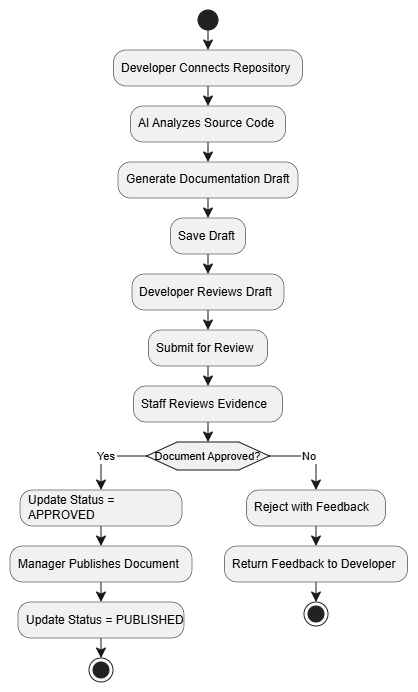
\includegraphics[width=\textwidth]{images/Activity_Diagram.png}
    \caption{AI Documentation Generation Activity Diagram}
    \label{fig:activity-ai}
\end{figure}

%================================================

\section{Component Responsibilities}

\begin{longtable}{|p{4cm}|p{8cm}|}
\hline
\textbf{Component} & \textbf{Responsibility}\\
\hline
GitHub Integration & Receives repository events through Webhooks.\\
\hline
Source Parser & Reads project files and extracts syntax information.\\
\hline
AST Engine & Builds Abstract Syntax Trees for supported languages.\\
\hline
Context Builder & Creates semantic context for AI processing.\\
\hline
RAG Pipeline & Retrieves relevant documentation before generation.\\
\hline
LLM Generator & Produces technical documentation drafts.\\
\hline
Review Engine & Sends generated drafts to human reviewers.\\
\hline
Version Manager & Stores document versions and audit history.\\
\hline
\end{longtable}

%================================================

\section{AST-Based Analysis}

Instead of relying only on raw source code, LivingDocs first constructs an Abstract Syntax Tree (AST).

The AST enables the system to identify:

\begin{itemize}
    \item Classes
    \item Functions
    \item Parameters
    \item Return types
    \item Dependencies
    \item Structural relationships
\end{itemize}

This structured representation improves documentation accuracy compared with plain-text generation.

%================================================

\section{Retrieval-Augmented Generation}

The RAG pipeline enriches prompts with existing documentation before AI generation.

The process consists of:

\begin{enumerate}
    \item Retrieve related documentation.
    \item Combine retrieved context with AST information.
    \item Generate updated documentation.
    \item Return grounded output.
\end{enumerate}

Grounding evidence is displayed so reviewers can verify every generated section.

%================================================

\section{Output Verification}

Every generated document includes:

\begin{itemize}
    \item Source code references.
    \item Version information.
    \item Generation timestamp.
    \item Review status.
\end{itemize}

This design ensures that AI-generated content remains transparent and verifiable before publication. 
\chapter{Documentation Drift Detection}

\section{Overview}
The \textbf{Documentation Drift Detection} module within the LivingDocs system is designed to automatically identify inconsistencies (drift) between source code hosted on GitHub and its associated documentation. Whenever code changes occur via commits or Pull Requests, the system parses the code, performs semantic evaluation, and compares it against existing documentation to issue timely alerts.

This module aligns with the functional specifications defined in the system requirement documentation.

\section{Objectives \& Scope}
\begin{itemize}
    \item Intercept and process commit and Pull Request events via GitHub Webhooks.
    \item Analyze source code structure using Abstract Syntax Tree (AST) parsing and semantic analysis.
    \item Map and compare code entities with existing documentation artifacts.
    \item Calculate drift confidence scores and classify severity levels (Low, Medium, High, Critical).
    \item Automatically generate drift reports with grounding evidence and dispatch alerts to Staff and Technical Leads.
\end{itemize}

\section{Functional Details}

\subsection{GitHub Event Ingestion (FR01)}
The system uses Webhooks to receive real-time updates whenever a new commit is pushed or a Pull Request is opened or updated in a monitored repository.

\subsection{AST Source Code Parsing (FR02)}
Modified source code is processed through an AST parser to extract key technical entities:
\begin{itemize}
    \item Class names, method signatures, interfaces, and package hierarchies.
    \item Input parameter lists, data types, return values, and exceptions.
    \item Associated docstrings, inline comments, and annotations.
\end{itemize}

\subsection{Code-Doc Comparison \& Scoring (FR03, FR04)}
The system retrieves documentation linked to the modified source files and evaluates consistency across three drift categories:
\begin{itemize}
    \item \textbf{Referential Drift:} Referenced classes, methods, or parameters have been deleted, moved, or renamed.
    \item \textbf{Signature Drift:} Method signatures, parameters, or return types have changed while the name remains identical.
    \item \textbf{Semantic Drift:} Internal business logic or component behavior has changed while signatures remain unchanged.
\end{itemize}

Drift severity is classified into four levels:
\begin{itemize}
    \item \textbf{Low (No/Minor Drift):} Cosmetic changes, inline comment fixes, or internal variable renames.
    \item \textbf{Medium (Moderate Drift):} Internal logic updates affecting module behavior without breaking external contracts.
    \item \textbf{High (Signature Drift):} Altered function parameters or return signatures not yet updated in docs.
    \item \textbf{Critical (Breaking Drift):} Deleted/renamed core APIs, major architectural refactoring, or critical config changes.
\end{itemize}

\subsection{Report Generation \& Alerting (FR05, FR06)}
The system automatically generates a detailed drift report comprising:
\begin{itemize}
    \item Commit hash or Pull Request ID.
    \item Affected source files and corresponding documentation links.
    \item Grounding evidence (Code Diff, Commit context, and Jira ticket metadata).
    \item Drift severity level, AI confidence score, and suggested update draft.
\end{itemize}
Alerts are delivered to Staff reviewers or Technical Leads via the system web interface, Slack, or email notifications.

\section{Processing Workflow}
\begin{verbatim}
  GitHub Event (Commit / PR)
              |
              v
     AST & Semantic Analysis
              |
              v
  Code-to-Doc Knowledge Retrieval
              |
              v
   Drift Scoring & Classification
              |
              v
 Report Generation & Notification Dispatch
\end{verbatim}

\section{Acceptance Criteria}
\begin{enumerate}
    \item Accurately receive and process Webhook event payloads from GitHub.
    \item Successfully parse modified source code and extract code entities via AST.
    \item Correctly detect and classify drift severity (Referential, Signature, Semantic).
    \item Generate comprehensive drift reports accompanied by grounding evidence and alert designated reviewers.
\end{enumerate}
\chapter{Automatic Documentation Update on Source-Code Change}

Documentation drift occurs frequently in software engineering when code evolves continuously through Commits and Pull Requests while technical documentation remains untouched. The \textbf{Automatic Documentation Update} module in LivingDocs addresses this issue by automatically maintaining synchronization between source code changes and project documentation.

\section{Module Overview \& Objectives}
The primary objective of this module is to automate the end-to-end process of detecting code modifications and updating affected documentation artifacts:
\begin{itemize}
    \item \textbf{Real-Time Event Detection:} Intercept source code modification events dispatched via GitHub Webhooks (Push Commits, PR creations/updates, and PR merges).
    \item \textbf{AST \& AI-Driven Generation:} Utilize Abstract Syntax Tree (AST) parsing alongside LLM and RAG capabilities to identify affected code entities (Classes, Methods, Endpoints, Parameters) and draft updated documentation versions.
    \item \textbf{Governed Workflow Integration:} Route automatically updated documentation drafts into the multi-tiered approval pipeline (AI $\rightarrow$ Staff Reviewer $\rightarrow$ Manager Approver) prior to publishing.
    \item \textbf{Side-by-Side Diff \& Rollback:} Provide interactive side-by-side diff views, track version change logs, and enable single-click version rollbacks.
\end{itemize}

\section{Functional Requirements}

\begin{table}[h!]
\centering
\small
\caption{Functional Requirements Matrix for Automatic Documentation Update}
\vspace{0.5em}
\begin{tabularx}{\textwidth}{|l|p{3.8cm}|X|c|}
\hline
\textbf{Requirement ID} & \textbf{Feature Name} & \textbf{Functional Description} & \textbf{Priority} \\ \hline
\textbf{FR-AU-01} & Auto-Update Trigger & Automatically detect code changes via Commit/PR, identify affected docs, and generate draft versions. & Critical \\ \hline
\textbf{FR-AU-02} & Auto-Update Toggles & Enable or disable auto-update features per Repository, Module, or specific Document type. & High \\ \hline
\textbf{FR-AU-03} & Auto-Updated View & Display a list of documentation drafts automatically updated by the AI engine following code changes. & High \\ \hline
\textbf{FR-AU-04} & Grounding Evidence Linkage & Link each auto-updated document draft to its triggering Commit Hash, Author, and Code Diff. & High \\ \hline
\textbf{FR-AU-05} & Side-by-Side Diff View & Provide a visual line-by-line diff comparing the AI-generated draft against the currently published version. & Critical \\ \hline
\textbf{FR-AU-06} & Developer Actions & Allow developers to Accept (forward to review), Edit directly, or Dismiss AI-suggested updates. & Critical \\ \hline
\textbf{FR-AU-07} & On-Demand Re-update & Allow developers to manually trigger re-generation for a specific code entity's documentation when required. & Medium \\ \hline
\textbf{FR-AU-08} & Document Rollback & Enable authorized users to roll back a document to the state prior to an auto-update execution. & Critical \\ \hline
\end{tabularx}
\end{table}

\section{Detailed Use Cases}

\subsection{UC-AU-01: Automatic Update Triggering on Source Code Change}
\begin{itemize}
    \item \textbf{Actors:} System (GitHub Webhook / Event Bus), Developer.
    \item \textbf{Pre-conditions:} The repository is connected to LivingDocs and auto-update policies are active.
    \item \textbf{Main Flow:}
    \begin{enumerate}
        \item GitHub sends a webhook payload (\texttt{push} or \texttt{pull\_request}) upon code changes.
        \item The \texttt{CodeAnalysisService} parses AST diffs to identify modified code entities.
        \item The \texttt{RagRetrievalService} queries the Knowledge Base to locate linked documentation chunks.
        \item The AI Engine processes the Code Diff, Document Context, and Template rules to generate an updated draft.
        \item The system stores the draft under \texttt{PENDING\_DEV\_ACCEPTANCE} status and notifies the developer.
    \end{enumerate}
\end{itemize}

\subsection{UC-AU-02: Diff Comparison \& Developer Acceptance}
\begin{itemize}
    \item \textbf{Actors:} Developer / Author.
    \item \textbf{Pre-conditions:} An AI auto-updated draft is pending review.
    \item \textbf{Main Flow:}
    \begin{enumerate}
        \item The developer opens the side-by-side diff view.
        \item The interface highlights added, modified, or removed sections.
        \item The developer executes one of the following actions:
        \begin{itemize}
            \item \textbf{Accept:} Approves the draft and forwards it to the Staff Review Queue.
            \item \textbf{Edit:} Modifies the Markdown draft directly before submitting.
            \item \textbf{Dismiss:} Rejects the AI proposal if no documentation update is necessary.
        \end{itemize}
    \end{enumerate}
\end{itemize}

\section{System Architecture \& Processing Flow}
The auto-update module relies on an event-driven microservices architecture:

\begin{verbatim}
[GitHub Webhook] ---> (POST /api/v1/webhooks/github) ---> [Spring Boot Backend]
  1. Validate HMAC signature & extract Commit SHA / Code Diff.
  2. Publish message to Kafka Topic: "code-change-events".

[Kafka Consumer] ---> [Python AI Engine (FastAPI)]
  1. Parse AST to detect function signature/behavioral changes.
  2. Execute RAG to pull relevant documentation chunks.
  3. Prompt LLM to update documentation maintaining template structure.

[Spring Boot Backend]
  1. Persist new record in `document_versions` with status 'PENDING_DEV'.
  2. Create audit trail record in `document_change_logs`.
  3. Dispatch WebSocket notification to developer interface.
\end{verbatim}

\section{Database Schema}
The module maintains history, change logs, and configuration state using PostgreSQL tables:

\begin{lstlisting}[language=SQL, caption={PostgreSQL Database Schema for Auto Update Module}]
-- Document Versions Entity
CREATE TABLE document_versions (
    id UUID PRIMARY KEY DEFAULT gen_random_uuid(),
    document_id UUID NOT NULL REFERENCES documents(id) ON DELETE CASCADE,
    version_number VARCHAR(20) NOT NULL,
    content TEXT NOT NULL,
    created_by_role VARCHAR(20) NOT NULL, -- 'AI', 'DEVELOPER', 'STAFF', 'MANAGER'
    trigger_type VARCHAR(30) NOT NULL,    -- 'COMMIT', 'PULL_REQUEST', 'ROLLBACK'
    trigger_commit_hash VARCHAR(40),
    confidence_score FLOAT,
    status VARCHAR(30) NOT NULL,          -- 'PENDING_DEV', 'IN_REVIEW', 'PUBLISHED'
    created_at TIMESTAMP WITH TIME ZONE DEFAULT CURRENT_TIMESTAMP
);

-- Audit & Change Log Entity
CREATE TABLE document_change_logs (
    id UUID PRIMARY KEY DEFAULT gen_random_uuid(),
    document_id UUID NOT NULL REFERENCES documents(id) ON DELETE CASCADE,
    from_version_id UUID REFERENCES document_versions(id),
    to_version_id UUID REFERENCES document_versions(id),
    acting_role VARCHAR(20) NOT NULL,     -- 'AI', 'STAFF', 'MANAGER'
    action_type VARCHAR(50) NOT NULL,     -- 'AUTO_UPDATE_GENERATED', 'ROLLBACK'
    change_summary TEXT,
    grounding_evidence JSONB,
    created_at TIMESTAMP WITH TIME ZONE DEFAULT CURRENT_TIMESTAMP
);
\end{lstlisting}
\chapter{Knowledge Base \& Vector Retrieval Management}

The \textbf{Knowledge Base} serves as the central semantic memory for the LivingDocs system. It is responsible for indexing, vectorizing, and retrieving documentation chunks to support Retrieval-Augmented Generation (RAG) during automated documentation updates and drift detection workflows.

\section{Module Overview \& Objectives}
The Knowledge Base module manages both raw documentation artifacts and their high-dimensional vector embeddings to enable fast, accurate semantic searches. Key functional objectives include:
\begin{itemize}
    \item \textbf{Automated Chunking \& Ingestion:} Parse incoming Markdown/LaTeX documentation into semantic chunks and generate vector embeddings via embedding models.
    \item \textbf{Vector Store Management:} Index chunk embeddings into a high-performance vector database (e.g., Qdrant / Pgvector) for efficient similarity searches.
    \item \textbf{Semantic RAG Retrieval:} Retrieve relevant context based on code diff keywords, Abstract Syntax Tree (AST) entities, and natural language queries.
    \item \textbf{Audit Trail \& History Tracking:} Maintain full version lineage for each knowledge chunk to support change auditing and seamless version rollbacks.
\end{itemize}

\section{Functional Requirements Matrix}

\begin{table}[h!]
\centering
\small
\caption{Functional Requirements for Knowledge Base Module}
\vspace{0.5em}
\begin{tabularx}{\textwidth}{|l|p{3.8cm}|X|c|}
\hline
\textbf{Requirement ID} & \textbf{Feature Name} & \textbf{Functional Description} & \textbf{Priority} \\ \hline
\textbf{FR-KB-01} & Document Indexing & Automatically chunk and vectorize updated or newly published documents into the Vector Store. & Critical \\ \hline
\textbf{FR-KB-02} & Hybrid Semantic Search & Execute combined dense (vector) and sparse (keyword) queries to fetch grounding context for LLM generation. & Critical \\ \hline
\textbf{FR-KB-03} & Linkage Mapping & Maintain bidirectional mappings between code AST symbols (classes, functions) and document chunks. & High \\ \hline
\textbf{FR-KB-04} & Chunk Versioning & Track chunk-level history, maintaining active/deprecated states for out-of-date knowledge. & High \\ \hline
\textbf{FR-KB-05} & Knowledge Maintenance & Provide APIs for manual or automated re-indexing and pruning of stale vector embeddings. & Medium \\ \hline
\end{tabularx}
\end{table}

\section{Knowledge Processing \& Retrieval Pipeline}

\subsection{Document Ingestion Flow}
When a document is modified or auto-updated, the Knowledge Base ingestion pipeline executes the following steps:
\begin{enumerate}
    \item \textbf{Preprocessing \& Parsing:} Parse document syntax (Markdown / LaTeX) and break text into optimal semantic chunks (250–500 tokens with overlapping boundaries).
    \item \textbf{Embedding Generation:} Pass extracted chunks to the embedding model to produce 1536-dimensional vector representations.
    \item \textbf{Metadata Attachment:} Associate each chunk vector with metadata including \texttt{document\_id}, \texttt{version\_id}, \texttt{file\_path}, and linked \texttt{ast\_entities}.
    \item \textbf{Vector Upsert:} Store vectors and payload metadata in the Vector Store.
\end{enumerate}

\subsection{RAG Retrieval Sequence}
\begin{verbatim}
  [AST / Code Diff Trigger] 
             |
             v
 [Extract Key Entities & Context]
             |
             v
  [Generate Query Embedding]
             |
             v
  [Vector Search (Cosine Similarity)] ---> [Filter Stale Versions]
             |
             v
  [Top-K Document Chunks] ---> [Inject into LLM Prompt Context]
\end{verbatim}

\section{Database Schema}
The Knowledge Base relies on PostgreSQL (with \texttt{pgvector} extension) or dedicated vector databases to manage chunk metadata and version relations.

\begin{lstlisting}[language=SQL, caption={PostgreSQL Database Schema for Knowledge Base Chunks}]
-- Knowledge Base Document Chunks
CREATE TABLE document_chunks (
    id UUID PRIMARY KEY DEFAULT gen_random_uuid(),
    document_id UUID NOT NULL REFERENCES documents(id) ON DELETE CASCADE,
    version_id UUID NOT NULL REFERENCES document_versions(id) ON DELETE CASCADE,
    chunk_index INT NOT NULL,
    content TEXT NOT NULL,
    embedding vector(1536), -- Vector embedding representation
    linked_symbols JSONB,   -- Stores AST entities: ["com.livingdocs.service.UserService"]
    is_active BOOLEAN DEFAULT TRUE,
    created_at TIMESTAMP WITH TIME ZONE DEFAULT CURRENT_TIMESTAMP
);

-- Index for Fast Vector Similarity Search (HNSW)
CREATE INDEX idx_document_chunks_embedding 
ON document_chunks 
USING hnsw (embedding vector_cosine_ops);
\end{lstlisting}
\chapter{System Administration (Administrator)}

The System Administration module plays a pivotal role in maintaining system operations, ensuring security and compliance, managing role-based access control, and configuring Artificial Intelligence (AI Engine) parameters for the entire \textbf{LivingDocs} platform.

\section{User Management \& Role-Based Access Control (RBAC)}
The system enforces a strict Role-Based Access Control (RBAC) model to regulate access permissions for every organization member:
\begin{itemize}
    \item \textbf{Account \& Role Governance:}
    \begin{itemize}
        \item Create, update, activate, or suspend user accounts within the system.
        \item Assign and adjust user roles across 5 permission levels: \textit{Developer (Author)}, \textit{Staff (Reviewer)}, \textit{Manager (Approver)}, \textit{Technical Lead (Documentation Owner)}, and \textit{Administrator}.
    \end{itemize}
    \item \textbf{Workspace \& Repository Management:}
    \begin{itemize}
        \item Define and allocate Workspaces for engineering teams.
        \item Grant repository access permissions to specific user groups or teams.
    \end{itemize}
\end{itemize}

\section{Platform \& Version Control System Integration}
Administrators are responsible for establishing secure connections with the Version Control System (VCS) infrastructure and third-party developer tools:
\begin{itemize}
    \item \textbf{GitHub App \& OAuth Connection Configuration:}
    \begin{itemize}
        \item Configure Client ID, Client Secret, and Private Keys for GitHub App and OAuth2/OIDC connections.
        \item Manage repository access scopes requested during the GitHub App installation.
    \end{itemize}
    \item \textbf{GitHub Actions \& Webhook Integration:}
    \begin{itemize}
        \item Set up Webhook URLs to receive real-time event payloads from GitHub (Commits, Pull Requests, Merge events).
        \item Manage Webhook Secret Keys to verify signature payload authenticity.
    \end{itemize}
    \item \textbf{External Tool Integrations:}
    \begin{itemize}
        \item Configure connections with task management tools (e.g., Jira) to extract issue context associated with code changes.
        \item Set up notification channels (Slack, Microsoft Teams) for documentation drift alerts and pending approval reviews.
    \end{itemize}
\end{itemize}

\section{AI Engine Service Configuration}
Administrators can fine-tune AI Engine parameters to balance documentation output accuracy and operational API costs:
\begin{itemize}
    \item \textbf{Language Models \& Embeddings:}
    \begin{itemize}
        \item Select Large Language Models (LLMs) used for code analysis and documentation generation (e.g., GPT-4o, Claude 3.5 Sonnet, or open-source models such as Llama 3).
        \item Configure Vector Embedding models used in Retrieval-Augmented Generation (RAG).
    \end{itemize}
    \item \textbf{AI Operational Parameters:}
    \begin{itemize}
        \item \textit{Confidence Threshold:} Set minimum confidence scores required before AI can suggest documentation updates automatically.
        \item \textit{Token Budget:} Define token usage limits per task or workspace to manage LLM API expenditures.
        \item \textit{Supported Languages:} Manage the list of programming languages supported for Abstract Syntax Tree (AST) parsing (e.g., Java, Python, TypeScript, Go, C++).
    \end{itemize}
\end{itemize}

\section{Auto-Update Policies, Audit Logs \& System Operations}
\begin{itemize}
    \item \textbf{Auto-Update Governance:} Configure automatic documentation update triggers (on Commit, on PR, or on Merge) and set approval enforcement rules (route to Staff/Manager review vs. auto-apply after approval).
    \item \textbf{Change Log \& Audit Trail Retention:} Set retention policies for document version histories and system audit logs to support compliance and traceability.
    \item \textbf{System Monitoring \& Infrastructure Health:}
    \begin{itemize}
        \item Monitor runtime performance across Microservices (Spring Boot), AI Service (FastAPI), Message Broker (Kafka), and Database (PostgreSQL).
        \item Manage event queues and inspect Dead Letter Queues (DLQ) for failed background AI tasks recovery.
    \end{itemize}
\end{itemize}
\chapter{System Testing \& Quality Assurance Plan}

\section{Introduction}
Software testing is a critical phase in the software development lifecycle, ensuring that the system operates strictly according to functional requirements, meets established quality benchmarks, and minimizes potential operational defects prior to production release. 

For the \textbf{LivingDocs} platform, quality assurance plays an indispensable role due to the system's architecture, which integrates multiple loosely coupled modules: GitHub Webhook Integration, AST Parsing, Retrieval-Augmented Generation (RAG), Vector Databases, and Multi-Tier Governance Workflows. An unhandled exception or data mismatch in any upstream module can compromise automated documentation synchronization.

This chapter outlines the comprehensive testing strategy, environmental configurations, test scenarios, and concrete execution results designed to validate the LivingDocs platform.

\section{Testing Objectives \& Scope}

\subsection{Testing Objectives}
The quality assurance process for LivingDocs is structured around the following goals:
\begin{itemize}
    \item \textbf{Functional Verification:} Ensure all core features operate as defined in the functional requirements matrix.
    \item \textbf{Integration Integrity:} Validate seamless data transfer across GitHub Webhooks, Spring Boot Core Services, Python AI Engines, and Vector Databases.
    \item \textbf{Accuracy of AI Generation:} Evaluate the precision and context alignment of documentation updates generated via RAG and LLM prompts.
    \item \textbf{Drift Detection Accuracy:} Verify the system's ability to accurately classify drift severity levels (Low, Medium, High, Critical) based on AST code changes.
    \item \textbf{Fault Tolerance \& Stability:} Test system behavior under error conditions, API rate limits, and unparseable source code diffs.
\end{itemize}

\subsection{Testing Scope}
The testing scope encompasses all functional modules of LivingDocs:
\begin{itemize}
    \item \textbf{GitHub Integration:} OAuth2 authentication, repository synchronization, and Webhook event delivery (Push, PR).
    \item \textbf{AST \& Code Analysis:} Abstract Syntax Tree parsing for detecting modified classes, method signatures, parameters, and return types.
    \item \textbf{Documentation Drift Detection:} Identification and severity scoring of Referential, Signature, and Semantic drifts.
    \item \textbf{AI Generation \& RAG Pipeline:} Vector search retrieval, prompt assembly, and Markdown documentation generation.
    \item \textbf{Automatic Documentation Update:} Automated draft generation, side-by-side diff comparison, and developer acceptance actions.
    \item \textbf{Review \& Approval Workflow:} Multi-tier governance routing (AI $\rightarrow$ Staff Reviewer $\rightarrow$ Manager Approver), comment logging, and publishing to GitHub.
    \item \textbf{Knowledge Base \& Versioning:} History tracking, change log audits, and single-click document rollback mechanisms.
\end{itemize}

\section{Testing Strategy \& Levels}

LivingDocs employs a multi-layered testing strategy to detect defects early and ensure system reliability:

\begin{itemize}
    \item \textbf{Unit Testing:} Conducted at the code level using JUnit 5 and Mockito for Java backend services, and PyTest for Python AI modules.
    \item \textbf{Integration Testing:} Validates API interactions, event consumption via Kafka, and database persistence between Spring Boot and FastAPI microservices.
    \item \textbf{System Testing:} End-to-end evaluation of complete workflows, simulating real GitHub Webhook payloads to final document publishing.
    \item \textbf{Acceptance Testing (UAT):} Execution of real-world scenarios to confirm the platform meets functional expectations for Developers, Staff Reviewers, and Managers.
\end{itemize}

\section{Testing Environment \& Tools}

Testing is conducted in an isolated environment mirroring the production setup to prevent data corruption and ensure reproducible results.

\begin{table}[h!]
\centering
\small
\caption{Testing Environment Specifications}
\vspace{0.5em}
\begin{tabularx}{\textwidth}{|l|X|}
\hline
\textbf{Component} & \textbf{Testing Technology / Configuration} \\ \hline
Backend Services & Java 17, Spring Boot 3.x, Python 3.11 (FastAPI) \\ \hline
Frontend Interface & ReactJS (TypeScript), TailwindCSS \\ \hline
Database Systems & PostgreSQL 15 (Metadata \& Versioning), Qdrant / Pgvector \\ \hline
Event Broker & Apache Kafka (Mocked/Local Container) \\ \hline
External API Mocks & Mock GitHub Webhook Payload Generator, OpenAI API Mocks \\ \hline
Testing Frameworks & JUnit 5, Mockito, PyTest, Postman, Jest \\ \hline
\end{tabularx}
\end{table}

\section{Defect Management Workflow}

Discovered bugs and discrepancies are processed through a structured lifecycle:
\begin{enumerate}
    \item \textbf{Logging:} Defects are logged with reproduction steps, error logs, and severity classifications.
    \item \textbf{Triage \& Assignment:} Issues are classified into severity levels (\textit{Critical, High, Medium, Low}) and assigned to the responsible module developer.
    \item \textbf{Remediation \& Retesting:} Fixed defects are deployed to the test environment and re-tested by QA.
    \item \textbf{Closure:} Once verified, the defect is officially marked as Closed.
\end{enumerate}

\section{Detailed Test Cases}

The following test cases demonstrate the execution and verification of key features within the \textbf{Documentation Drift Detection} and \textbf{Review Queue \& Approval Workflow} modules.

% ----------------- TEST CASE 1 -----------------
\paragraph{TC-RQ-001: Filter Review Queue Dashboard by Drift Severity}

\begin{longtable}{|l|p{10.5cm}|}
    \hline
    \textbf{Component} & \textbf{Test Case Specification} \\ \hline
    \textbf{Test ID} & TC-RQ-001 \\ \hline
    \textbf{Module} & Review Queue Dashboard \\ \hline
    \textbf{Objective} & Verify that the system correctly filters pending documentation reviews by their drift severity level (\textit{Critical, High, Medium, Low}). \\ \hline
    \textbf{Pre-conditions} & Staff reviewer is authenticated. The Review Queue contains at least 5 pending document drafts across various severity levels. \\ \hline
    \textbf{Input Data} & Select filter tag: \texttt{CRITICAL}. \\ \hline
    \textbf{Execution Steps} & 
    1. Navigate to the Review Queue Dashboard.\newline
    2. Locate the "Filter by Drift Severity" toolbar.\newline
    3. Click the \texttt{CRITICAL} severity filter button.\newline
    4. Observe the updated data grid. \\ \hline
    \textbf{Expected Result} & The queue updates immediately to show only items marked with \texttt{CRITICAL} severity (highlighted with a red badge). All other items are filtered out. \\ \hline
    \textbf{Actual Result} & Operating as expected (Verified on ReactJS prototype interface). \\ \hline
    \textbf{Status} & \textbf{\color{green}PASS} \\ \hline
\end{longtable}

\vspace{0.3cm}

% ----------------- TEST CASE 2 -----------------
\paragraph{TC-RQ-002: Staff Reviewer Evaluation and Approval}

\begin{longtable}{|l|p{10.5cm}|}
    \hline
    \textbf{Component} & \textbf{Test Case Specification} \\ \hline
    \textbf{Test ID} & TC-RQ-002 \\ \hline
    \textbf{Module} & Side-by-Side Review Workspace \\ \hline
    \textbf{Objective} & Verify that a Staff Reviewer can inspect side-by-side code/doc diffs, provide feedback, and approve a document from \texttt{IN\_REVIEW} to \texttt{APPROVED}. \\ \hline
    \textbf{Pre-conditions} & A document draft is in \texttt{IN\_REVIEW} status. User is logged in with Staff Reviewer privileges. \\ \hline
    \textbf{Input Data} & Feedback text: \textit{"Documentation matches modified API signatures accurately."}; Click \texttt{[Approve]} button. \\ \hline
    \textbf{Execution Steps} & 
    1. Click "Review" on a pending document entry in the Review Queue.\newline
    2. Inspect the Side-by-Side Workspace displaying Code Diff and Grounding Evidence.\newline
    3. Enter review feedback into the comment field.\newline
    4. Click the \texttt{[Approve]} button. \\ \hline
    \textbf{Expected Result} & 
    - Document status transitions from \texttt{IN\_REVIEW} to \texttt{APPROVED}.\newline
    - Toast notification appears: \textit{"Approved and forwarded to Manager successfully."}\newline
    - System redirects the user back to the active Review Queue. \\ \hline
    \textbf{Actual Result} & Operating as expected (Verified on ReactJS frontend linked with API mocks). \\ \hline
    \textbf{Status} & \textbf{\color{green}PASS} \\ \hline
\end{longtable}

\vspace{0.3cm}

% ----------------- TEST CASE 3 -----------------
\paragraph{TC-RQ-003: Final Manager Approval and GitHub Publication}

\begin{longtable}{|l|p{10.5cm}|}
    \hline
    \textbf{Component} & \textbf{Test Case Specification} \\ \hline
    \textbf{Test ID} & TC-RQ-003 \\ \hline
    \textbf{Module} & Manager Approval \& GitHub Publishing Service \\ \hline
    \textbf{Objective} & Verify that a Manager can grant final approval to publish an \texttt{APPROVED} document directly to the GitHub repository. \\ \hline
    \textbf{Pre-conditions} & Document status is \texttt{APPROVED}. User is logged in with Manager role privileges. \\ \hline
    \textbf{Input Data} & Click \texttt{[Publish Document]} button on the Manager approval dashboard. \\ \hline
    \textbf{Execution Steps} & 
    1. Access the Manager Approval queue.\newline
    2. Select a target document in \texttt{APPROVED} state.\newline
    3. Click \texttt{[Publish Document]}. \\ \hline
    \textbf{Expected Result} & 
    - Document status updates to \texttt{PUBLISHED}.\newline
    - The backend invokes the GitHub API service to commit the updated Markdown file to the designated repository path.\newline
    - An Audit Trail log entry is created recording the Manager ID, timestamp, and commit hash. \\ \hline
    \textbf{Actual Result} & Operating as expected (Verified with simulated GitHub Webhook/API integration). \\ \hline
    \textbf{Status} & \textbf{\color{green}PASS} \\ \hline
\end{longtable}

\section{Summary}
The testing framework established for LivingDocs guarantees that every component—from GitHub event ingestion to AI generation and multi-tier approval—is systematically verified. The successful execution of test cases demonstrates that the system achieves high reliability, accurate drift detection, and governed documentation maintenance.
\section{Conclusion}

\subsection{Project Summary}
In the context of modern software development, maintaining technical documentation that is always synchronized with source code is a major challenge for development teams. Many projects face the issue of documentation quickly becoming outdated due to infrequent updates, causing difficulties in maintenance, expansion, and system handover.

The \textbf{LivingDocs} project was proposed to address this problem by combining modern technologies such as GitHub Integration, Artificial Intelligence (AI), Retrieval-Augmented Generation (RAG), and Workflow Automation. The system aims to automate the creation, updating, and management of technical documentation based on source code changes, thereby significantly reducing manual workload and improving documentation quality.

Within the scope of the Software Engineering course, the team conducted requirement analysis, designed the overall architecture, and developed descriptive documentation for the main system components. These deliverables form the foundation for future development and deployment phases.

\subsection{Project Achievements}
During the project, the team accomplished the following key tasks:
\begin{itemize}
    \item Analyzed functional and non-functional requirements of the system.
    \item Designed GitHub integration workflow using OAuth2 and GitHub API.
    \item Built an automated documentation update process triggered by GitHub events.
    \item Proposed an AI architecture to support source code analysis and technical documentation generation.
    \item Designed a version management mechanism for documentation and detection of inconsistencies between documentation and source code.
    \item Developed testing procedures and a system quality evaluation plan.
\end{itemize}

These results contribute to forming a modern documentation management model that effectively supports software development in a systematic way.

\subsection{Project Limitations}
Due to time constraints and the scope of the course, the project still has certain limitations:
\begin{itemize}
    \item The system remains at the design and solution description stage, without full implementation of all functions.
    \item Some components such as the AI Engine, Vector Database, and Workflow Automation have not been tested in real environments.
    \item Performance, scalability, and security evaluations have not yet been conducted.
    \item Full integration with CI/CD processes in real development environments has not been implemented.
\end{itemize}

These limitations will serve as the basis for further improvement in subsequent development phases.

\subsection{Future Development}
In the future, the LivingDocs system can be expanded in various directions to enhance usability and practical application. Potential development directions include:
\begin{itemize}
    \item Full implementation of Backend, Frontend, and Database components.
    \item Integration of AI models with more accurate source code analysis capabilities.
    \item Extending support to multiple source code management platforms such as GitLab or Bitbucket.
    \item Adding automated testing and continuous deployment (CI/CD) mechanisms.
    \item Developing a more detailed role-based access control system.
    \item Optimizing system performance for large-scale projects.
    \item Strengthening security and monitoring solutions during operation.
\end{itemize}

Advancing along these directions will help LivingDocs become an intelligent technical documentation management platform, better meeting the needs of real-world software development teams.

\subsection{Conclusion}
Overall, the \textbf{LivingDocs} project has proposed a solution to support technical documentation management in an automated, intelligent, and synchronized manner with the software development process. Through GitHub integration, AI application, and workflow automation, the system aims to reduce manual work, improve documentation accuracy, and enhance collaboration efficiency within development teams.

Although the project is currently at the design and documentation stage, the achieved results demonstrate the feasibility of the solution and lay the groundwork for future implementation. With the proposed development directions, LivingDocs has the potential to become a modern documentation management tool, contributing to improved quality in software development and maintenance in real-world projects.


% --- TÀI LIỆU THAM KHẢO ---
% Liên kết tự động tới file references.bib trong thư mục docs/
\bibliographystyle{IEEEtran}
\bibliography{references}

\end{document}